\documentclass[11pt,a4paper,twocolumn]{article}

% === Core Packages ===
\usepackage[margin=2cm]{geometry}
\usepackage[utf8]{inputenc}
\usepackage[T1]{fontenc}
\usepackage{times}
\usepackage{amsmath,amssymb}
\usepackage{graphicx}
\usepackage{booktabs}
\usepackage{float}
\usepackage{enumitem}
\usepackage{tikz}
\usepackage{pgfplots}
\pgfplotsset{compat=1.18}
\usetikzlibrary{arrows.meta,shapes.geometric,positioning,calc,decorations.markings,fit,backgrounds}

% === Citation (IEEE style) ===
\usepackage[numbers,sort&compress]{natbib}
\bibliographystyle{IEEEtranN}

% === Hyperref ===
\usepackage[hidelinks]{hyperref}
\usepackage{xurl}

% === Settings ===
\setlength{\parindent}{1em}
\setlength{\parskip}{0.3em}

% === PDF metadata ===
\hypersetup{
  pdftitle={Merkeziyetsiz İtibar Ağı: Doğal Toplumsal Örgütlenme İçin Bir Çerçeve},
  pdfauthor={Pavel Kudrna},
  pdfsubject={Personix — a decentralized reputation network},
  pdfkeywords={Personix, decentralized reputation, reputation social network,
    decentralized identifiers, DID, meritocracy, censorship resistance},
}

% === Title ===
\title{\textbf{Merkeziyetsiz İtibar Ağı:\\Doğal Toplumsal Örgütlenme İçin Bir Çerçeve}}
\author{Pavel Kudrna\\Personix Project --- \url{https://personix.org}\\Prague, Czechia\\Draft v1 --- March 2026}
\date{}

\begin{document}
\maketitle

% ============================================================
% ABSTRACT
% ============================================================
\begin{abstract}
Adalet duygusu---haksızlıkların düzeltildiği ve liyakatin ödüllendirildiği inancı---toplumun en güçlü birleştirici gücüdür. Bir hakkı uygulamanın maliyeti hakkın kendisinin değerini aştığı için merkezî yönetim kurumları bu duyguyu sağlayamadığında, toplumsal uyum aşınır. Mevcut kurumsal yapılar, önemli bir uyuşmazlık sınıfını, merkezî planlamanın kaynakları tahsis etmekte başarısız olmasıyla sistematik olarak aynı biçimde çözmekte başarısız olur: bilgi asimetrisi, eksik geri bildirim döngüleri ve karar vericilerin kararlarının sonuçlarından kopukluğu yoluyla. Bu makale bir İtibar Sosyal Ağı (RSN) sunar: Merkeziyetsiz Kimlik Belirteçleri (DID) üzerine kurulu, takma adlı katılımcıların gerçek dünyadaki davranışlar hakkındaki itibar bilgilerini yayımlamasını, doğrulamasını ve tüketmesini sağlayan merkeziyetsiz, yozlaştırılamaz, sansüre dirençli bir iletişim katmanı. Temel mekanizma üç tasarım ilkesine dayanır: (1)~itibar verilerini okumanın ucuz olduğu ancak yazmanın doğrulanabilir çaba gerektirdiği asimetrik bir maliyet yapısı; (2)~radikal iddiaları giderek artan yineleme maliyetleri aracılığıyla fiyatlandıran, tutarlı özetlemeye (consistent hashing) dayalı deterministik olmayan bir doğrulayıcı seçim protokolü; ve (3)~özel doğrulayıcıların onayladıkları iddiaların doğruluğuna biriktirdikleri itibarı ortaya koydukları, piyasa güdümlü bir itibar otoritesi modeli. Ortaya çıkan mimari, merkezî koordinasyon olmaksızın kendiliğinden bir liyakat sistemi üretir ve mevcut devlet tarafından yönetilen sistemlerden kademeli, geri döndürülebilir bir geçiş yolu sağlar.
\end{abstract}

% ============================================================
% 1. INTRODUCTION
% ============================================================
\section{Giriş}

\subsection{Merkezî Güvenin Sorunu}

Modern yönetim temel bir varsayıma dayanır: merkezî kurumların, yabancılar arasındaki güveni ölçekte aracılık edebileceği. Mahkemeler uyuşmazlıkları çözer. Siciller mülkiyeti belgeler. Düzenleyici kurumlar standartları uygular. Bu kurumlar, bilginin kıt olduğu, iletişimin yavaş olduğu ve yetkinin merkezî bir organa devredilmesinin tek uygulanabilir koordinasyon mekanizması olduğu bir çağda tasarlanmıştı. Ancak merkezî yönetim, merkezî planlamayla aynı yapısal nedenlerle başarısız olur: bilgi asimetrisi, eksik geri bildirim döngüleri ve karar vericilerin kararlarının sonuçlarından kopukluğu.

Bu varsayım, örneğin kurumsal aracılığın maliyeti uyuşmazlığın değerini aştığında başarısız olur. Kiraladığı dairenin yasal olarak zorunlu bir elektrik güvenliği belgesinden yoksun olduğunu keşfeden bir kiracıyı düşünün---hayat için doğrudan tehlike oluşturan bir durum. Kiracının sözleşmeden çekilme yönündeki yasal hakkı tartışmasızdır. Ancak bu hakkı mahkeme sistemi aracılığıyla uygulamanın maliyeti, potansiyel yasal tazminat dahil olmak üzere, depozitonun ve alacaklı olunan zararların parasal değerini aşar~\cite{czcourtfees}. Rasyonel yanıt, kaybı üstlenmek ve çıkmaktır.

Bu, patolojik bir uç durum değildir. Zararın gerçek olduğu ancak parasal riskin, kurumsal uygulamanın ekonomik olarak rasyonel hale geldiği eşiğin altına düştüğü önemli bir uyuşmazlık sınıfı için varsayılan deneyimdir. Sonuç, kötü niyetli aktörleri yapısal olarak kayıran bir sistemdir: başkalarına bu eşiğin altındaki hacimlerde zarar verenler cezasız kalabilir, çünkü adalet arama maliyeti zarar gören tarafa düşer.

Yukarıdaki örnek, yazarın hukukî ortamından---Çek medenî hukuk sisteminden---alınmıştır. Diğer hukuk geleneklerinde---içtihat temelli ortak hukuk (common law), örf ve âdet hukuku, karma sistemler---adalet, yargı çevresinin kültürel ve usulî özelliklerine bağlı olarak farklı biçimlerde ve farklı derecelerde başarısız olur. Okurlar muhtemelen kendi bağlamlarından eşdeğer örnekler tanıyacaklardır. Yapısal olarak evrensel olan örüntüdür: değeri ekonomik olarak rasyonel uygulama eşiğinin altına düşen uyuşmazlıklar, kaybın zarar gören tarafça üstlenilmesiyle son bulur. RSN mükemmel adalet vaat etmez---yalnızca kurumsal uygulamanın ekonomik olmadığı durumlarda kötü niyetli aktörlerin sahip olduğu yapısal avantajı azaltır.

\subsection{Mevcut Çözümler Neden Yetersiz Kalıyor}

\textbf{Merkeziyetsiz Kimlik (DID) çerçeveleri}~\cite{did2022} öz-egemen kimlik yönetimi için kriptografik mekanizmalar sağlar ancak öncelikle kimlik doğrulamaya odaklanır ve davranışsal itibarın daha geniş sorununu ele almaz.

\textbf{Ruha Bağlı Belirteçler (SBT'ler)}~\cite{weyl2022} itibarın devredilemez olduğu içgörüsünü yakalar ancak ölçeklenebilirlik kısıtlamaları olan blok zinciri altyapısına dayanır ve bilgi girişini yöneten ekonomik teşvikleri ele almaz. Liyakat belirteçleri (ör. Liberland) gibi ilgili kavramlar benzer bir felsefeyi paylaşır ancak belirli yargı çerçevelerine bağlı kalır.

\textbf{Merkeziyetsiz Özerk Organizasyonlar (DAO'lar)}~\cite{buterin2014} yönetimi akıllı sözleşmeler aracılığıyla uygular ancak etkinin sermayeyle orantılı olduğu plütokratik dinamikleri yeniden üretir. Karesel oylama~\cite{buterin2019} bunu kısmen hafifletir ancak pratik benimsemeyi sınırlar. DAO'lar ayrıca temel \emph{kâhin (oracle) sorunuyla} karşı karşıyadır: akıllı sözleşmeler güvenilir bir dış kaynak olmadan gerçek dünya durumlarını güvenilir biçimde doğrulayamaz ve bu sorunun blok zinciri mimarisi içinde genel bir çözümü yoktur.

Mevcut hiçbir sistem merkeziyetsizliği, sansür direncini, takma adlılığı, doğrulanabilir giriş maliyetini ve kendiliğinden oluşan uzlaşıyı bir arada barındırmaz.

\subsection{Katkılar}

Bu makale şu katkıları sunar:
\begin{enumerate}[nosep]
\item DID çerçevesini iki yönlü itibar değişimini destekleyecek şekilde genişleten merkeziyetsiz bir protokol olan \textbf{İtibar Sosyal Ağı'nın (RSN)} tanımı.
\item Tutarlı özetlemeye dayalı \textbf{deterministik olmayan bir doğrulayıcı seçim protokolü}~\cite{karger1997}.
\item İddiaları, üç bileşik maliyet kanalı aracılığıyla ağ uzlaşısından uzaklıklarına göre fiyatlandıran \textbf{Pahalı Radikallik İlkesi}.
\item Sahte onayın maliyetinin meşru ücretlerden felaket derecesinde daha fazla olduğu, asimetrik teşviklere sahip bir \textbf{İtibarlı Otorite modeli}.
\item Paralel malî altyapı aracılığıyla \textbf{kademeli bir geçiş yolu}.
\end{enumerate}

% ============================================================
% 2. DESIGN PRINCIPLES
% ============================================================
\section{Tasarım İlkeleri}

RSN mimarisi, pazarlığa açık olmayan beş tasarım ilkesiyle kısıtlanmıştır.

\textbf{Süreklilik ve Evrim.} Sistem, belirsiz uzunlukta bir geçiş döneminde mevcut kurumlarla bir arada var olur. Geçiş her aşamada geri döndürülebilir olmalıdır.

\textbf{Gönüllülük ve Sorumluluk.} Katılım gönüllüdür ancak gönüllülük sorumlulukla eşleşir: kurumsal bir işlev üzerinde denetim üstlenen bir katılımcı, eşzamanlı olarak beraberindeki yükümlülükleri de üstlenir.

\textbf{Çeşitlilik ve Kültürel Tarafsızlık.} Uzlaşı, sistem tasarımcıları tarafından dayatılan önceden belirlenmiş kurallardan değil, iki yönlü etkileşimlerden ortaya çıkar.

\textbf{Dayanıklılık ve Sansür Direnci.} Ağı sansürlemenin maliyeti, ona katlanmanın maliyetini aşmalıdır. Sistemi yalnızca tam totaliterlik---yıkıcı siyasî ve ekonomik maliyetle---bastırabilir.

\textbf{Uzlaşı ve Uygulama.} Sistem, insanın küçüklük, kin ve intikam alma tatminine yönelik eğilimlerini taşıyıcı özellikler olarak bünyesine katar. Kötü davranış yasaklanmaz; fiyatlandırılır.

% ============================================================
% 3. SYSTEM OVERVIEW
% ============================================================
\section{Sisteme Genel Bakış}

\subsection{İtibar Sosyal Ağı}

RSN, katılımcıların gerçek dünyadaki davranışlar hakkında doğrulanabilir bilgi alışverişinde bulunduğu merkeziyetsiz, uçtan uca (peer-to-peer) bir iletişim katmanıdır. Tanımlayıcı özellikleri şunlardır: merkeziyetsiz ve sansürlenemez altyapı; DID'ler aracılığıyla takma adlı katılım; asimetrik maliyet yapısı (okumak ucuz, yazmak pahalıdır); kriptografik doğrulanabilirlik; ve \textbf{standart desteği}---ağ üzerinden yayılan bilgiler için, otoriteler tarafından sunulan hizmetler için (iddia oluşturma, onaylama, tanık hizmeti) ve karşı taraf itibarını değerlendirme kurallarını ve politika uyumsuzluğu riskini (beyan edilen ile fiilî davranış arasında) değerlendirmeyi içeren politika biçimi için makinece okunabilir formatlar.

\subsection{Mimarî Bileşenler}

RSN dört ana bileşenden oluşur (Şek.~\ref{fig:architecture}):
\begin{enumerate}[nosep]
\item \textbf{DID Katmanı.} Beyan edilen kurallar, itibar meta verileri ve ağ yönlendirmesi ile katılımcı kimlikleri.
\item \textbf{İddia Protokolü.} Gerçek dünya olayları hakkındaki iddiaları yayımlamak için yapılandırılmış format.
\item \textbf{Doğrulama Ağı.} Tutarlı özetleme kullanarak doğrulayıcı atamaya yönelik merkeziyetsiz protokol.
\item \textbf{İtibar Toplama Katmanı.} İnsan tarafından okunabilir itibar özetleri üreten hizmetler.
\end{enumerate}

\begin{figure}[ht]
\centering
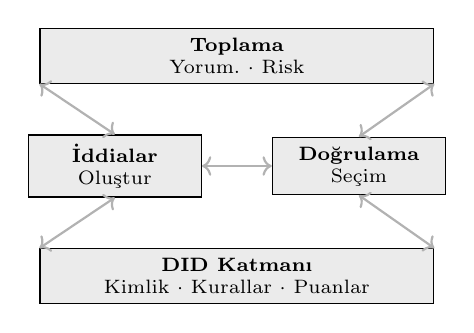
\begin{tikzpicture}[
    layer/.style={draw, minimum height=0.7cm, align=center, font=\scriptsize, fill=black!8},
    arr/.style={<->, thick, gray!60}
]
\node[layer, minimum width=5cm] (agg) at (0,2.8) {\textbf{Toplama}\\Yorum.\ $\cdot$ Risk};
\node[layer, minimum width=2.2cm] (claim) at (-1.55,1.4) {\textbf{İddialar}\\Oluştur};
\node[layer, minimum width=2.2cm] (verif) at (1.55,1.4) {\textbf{Doğrulama}\\Seçim};
\node[layer, minimum width=5cm] (did) at (0,0) {\textbf{DID Katmanı}\\Kimlik $\cdot$ Kurallar $\cdot$ Puanlar};

\draw[arr] (agg.south west) -- (claim.north);
\draw[arr] (agg.south east) -- (verif.north);
\draw[arr] (claim.east) -- (verif.west);
\draw[arr] (claim.south) -- (did.north west);
\draw[arr] (verif.south) -- (did.north east);
\end{tikzpicture}
\caption{RSN dört katmanlı mimarisi.}
\label{fig:architecture}
\end{figure}

\subsection{Katılımcı Rolleri}

Bir doğrulama işlemi en fazla altı farklı DID rolünü içerir (Şek.~\ref{fig:roles}): \textbf{İhraççı} ($DID_I$, iddiayı oluşturur ve sunar), \textbf{Özne} ($DID_S$, iddianın hakkında olduğu DID---İhraççı ile örtüşebilir), \textbf{Otorite} ($DID_A$, iddiayı bir ücret karşılığında onaylar; tanık hizmetleri de sunabilir---\emph{isteğe bağlı}), \textbf{Tanık} ($DID_{W_{1..n}}$, meydan okuma kodları aracılığıyla doğrulayıcı dürüstlüğünü gizlice izleyen---\emph{isteğe bağlı}), \textbf{Doğrulayıcı} ($DID_V$, iddiayı yayımlamak üzere algoritmik olarak seçilen) ve \textbf{RSN} (doğrulanmış iddiaların yayımlandığı ağ). Herhangi bir rol başka bir DID'e devredilebilir (Bölüm~7.4). Bir Otorite genellikle onaylamayı tanık hizmetleriyle birleştirir ancak bu iki işlev mantıksal olarak bağımsızdır.

\begin{figure}[ht]
\centering
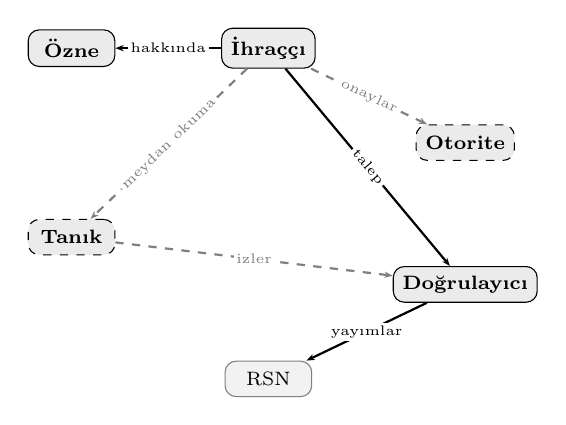
\begin{tikzpicture}[
    role/.style={draw, rounded corners, minimum width=1.1cm, minimum height=0.45cm, align=center, font=\scriptsize, fill=black!8},
    opt/.style={draw, rounded corners, minimum width=1.1cm, minimum height=0.45cm, align=center, font=\scriptsize, fill=black!8, dashed},
    arr/.style={-{Stealth[length=3pt]}, thick},
    oarr/.style={-{Stealth[length=3pt]}, thick, dashed, gray},
    lbl/.style={font=\tiny, fill=white, inner sep=1pt}
]
\node[role] (I) at (0,2.4) {\textbf{İhraççı}};
\node[role] (S) at (-2.5,2.4) {\textbf{Özne}};
\node[opt] (A) at (2.5,1.2) {\textbf{Otorite}};
\node[opt] (W) at (-2.5,0) {\textbf{Tanık}};
\node[role] (V) at (2.5,-0.6) {\textbf{Doğrulayıcı}};
\node[role, fill=black!5, draw=gray] (N) at (0,-1.8) {RSN};

\draw[arr] (I) -- node[lbl] {hakkında} (S);
\draw[oarr] (I) -- node[lbl,sloped] {onaylar} (A);
\draw[oarr] (I) -- node[lbl,sloped] {meydan okuma} (W);
\draw[arr] (I) -- node[lbl,sloped] {talep} (V);
\draw[oarr] (W) -- node[lbl] {izler} (V);
\draw[arr] (V) -- node[lbl] {yayımlar} (N);
\end{tikzpicture}
\caption{Bir doğrulama işlemindeki DID rolleri. Kesikli = isteğe bağlı (Otorite, Tanık).}
\label{fig:roles}
\end{figure}

\subsection{Yozlaştırılamazlık: Dört Güç}

RSN'nin yozlaştırılamazlığı tek bir mekanizmadan değil, eşzamanlı dört güçten kaynaklanır. Hiçbiri tek başına yeterli değildir; yalnızca bunların birleşimi yozlaştırma girişimini ekonomik olarak akıl dışı kılar.

\textbf{Öngörülemeyen hedef.} Her iddia için doğrulayıcı, tutarlı özetleme yoluyla deterministik olmayan biçimde seçilir (Bölüm~5.3). Bir saldırgan rüşvet için belirli bir doğrulayıcıyı önceden hedefleyemez, çünkü doğrulayıcının kimliği ihraççının seçiminin değil, iddianın içeriğinin ve önceki yinelemelerin bir işlevidir.

\textbf{İtibar kaldıracı---yavaş yükselir, hızlı düşer.} İtibar yalnızca kademeli olarak, sürekli tutarlı davranışla kazanılabilir. Ancak tek bir sahtekârca onayda felaket derecesinde kaybedilebilir (Bölüm~6.2). Bu asimetri, yıllarca biriktirilen itibarın tek bir sahtekârca onayla yok edilebileceği anlamına gelir; optimal strateji şüpheli iddiaları reddetmek olarak kalır.

\textbf{Kamusal vaat.} Her DID Sahibi kendi politikasını---uymayı taahhüt ettiği makinece okunabilir bir kurallar dizisini---kamuya açık olarak beyan eder. Beyan ile fiilî davranış arasındaki ayrışma tespit edilebilir ve temeldeki ihlalden daha ağır bir itibar suçu olarak fiyatlandırılır (Bölüm~7.3). Bu nedenle ikiyüzlülük, doğrudan sahtekârlıktan daha maliyetlidir.

\textbf{Örgü ağı saldırı-maliyet asimetrisi.} Ağı sansürleme veya istikrarsızlaştırma maliyeti ağın büyüklüğü ve yoğunluğuyla doğrusal olmayan biçimde artarken, ona katlanma maliyeti sabit kalır. Sansürün getiri sağlaması için merkezî bir aktörün bunu ağın tamamına uygulaması gerekir---düşünülebilecek herhangi bir yararla orantısız önlemler gerektirir (Bölüm~10).

% ============================================================
% 4. DECENTRALIZED IDENTITY MODEL
% ============================================================
\section{Merkeziyetsiz Kimlik Modeli}

\subsection{Özel Özelliklere Sahip DID}

RSN, W3C DID Core spesifikasyonunu~\cite{did2022} şu unsurlarla genişletir: \textbf{Beyan Edilen Kurallar} (makinece okunabilir davranışsal taahhütler), \textbf{İtibar Meta Verileri} (toplu davranışsal puan) ve \textbf{Ağ Yönlendirmesi} (kararlı halka konumundan ayrı, değiştirilebilir soğan geçidi).

\subsection{İddia Yaşam Döngüsü}

Bir İddia altı aşamadan geçer (Şek.~\ref{fig:lifecycle}): oluşturma, isteğe bağlı otorite onayı, tutarlı özetleme yoluyla doğrulayıcı seçimi, doğrulama kararı (kabul veya yinelemeyle ret), yayımlama ve tüm taraflar için itibar güncellemesi.

\begin{figure}[ht]
\centering
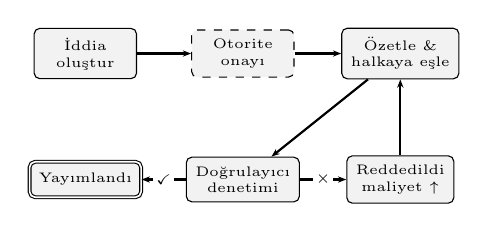
\begin{tikzpicture}[
    stp/.style={draw, rounded corners=2pt, minimum width=1.3cm, minimum height=0.45cm, align=center, font=\tiny, fill=black!5},
    arr/.style={-{Stealth[length=3pt]}, thick},
    lbl/.style={font=\tiny, fill=white, inner sep=1pt}
]
\node[stp] (comp) at (0,0) {İddia\\oluştur};
\node[stp, dashed] (auth) at (2.0,0) {Otorite\\onayı};
\node[stp] (hash) at (4.0,0) {Özetle \&\\halkaya eşle};
\node[stp] (ver) at (2.0,-1.6) {Doğrulayıcı\\denetimi};
\node[stp, double] (pub) at (0,-1.6) {Yayımlandı};
\node[stp] (rej) at (4.0,-1.6) {Reddedildi\\maliyet $\uparrow$};

\draw[arr] (comp) -- (auth);
\draw[arr] (auth) -- (hash);
\draw[arr] (hash) -- (ver);
\draw[arr] (ver) -- node[lbl] {\checkmark} (pub);
\draw[arr] (ver) -- node[lbl] {$\times$} (rej);
\draw[arr] (rej) -- ++(0,0.8) -| (hash);
\end{tikzpicture}
\caption{Yineleme döngülü iddia yaşam döngüsü.}
\label{fig:lifecycle}
\end{figure}

\subsection{W3C DID Core ile İlişki}

RSN'nin kimlik modeli, W3C DID Core spesifikasyonunun~\cite{did2022} tam bir üst kümesidir. Tüm RSN DID'leri geçerli W3C DID'leridir. RSN'ye özgü genişletmeler, ION~\cite{buchner2021} ve Ceramic~\cite{ceramic2023} gibi mevcut altyapılarla uyumlu, özel bir DID yöntemi spesifikasyonunda tanımlanan DID belgesi özellikleri olarak kodlanır.

% ============================================================
% 5. VERIFICATION AND PROPAGATION
% ============================================================
\section{Bilginin Doğrulanması ve Yayılması}

\subsection{Bilgi Girişinin Maliyeti}

RSN'nin temel ekonomik ilkesi, okuma ile yazma arasındaki asimetridir. İtibar verilerini okumak, DID ağının parçası olan ve itibarlarıyla orantılı erişime sahip katılımcılar için sıfır marjinal maliyete yaklaşır---yeni katılanlar daha geniş erişimi kademeli olarak hak etmelidir (bkz. asalaklığı önleme). Yazmak---tek seferlik bir teknik eylem olarak değil, itibarın ağa kalıcı biçimde maddeleşmesi olarak anlaşılan---üç boyutta doğrulanabilir birikimli yatırım gerektirir: \textbf{zaman} (tutarlı davranışa, yerine getirilen taahhütlere ve geliştirilen ilişkilere harcanan yıllar), \textbf{enerji} (dürüst ilişkilere, ortaklıklara özene ve uzun vadeli güvenilirliğe yatırılan çaba) ve \textbf{para} (kişinin kendi adına yatırımı---mesleki gelişim, işinin kalitesi, verilen zararların telafisi). İtibar anında satın alınamaz---sistemin yalnızca görünür ve bağlamlar arasında aktarılabilir kıldığı, yaşam boyu süren bir birikimin sonucudur. Protokolün tek seferlik teknik maliyetleri (kriptografik imzalar, doğrulayıcı ücretleri) bu temel yatırıma kıyasla ihmal edilebilir düzeydedir.

\subsection{Sosyal Grafik ve Bağlantı Derinliği}

RSN temelde bir sosyal ağdır: her DID, bağlantıya izin veren kişileri (diğer DID'leri) ekler. Bu bağlantıların kendi bağlantıları vardır ve bu böyle devam eder. Algoritmik doğrulayıcı araması, yapılandırılabilir bir $h$ derinliğindeki bağlı kişiler içinde çalışır (ör. $h=3$: kişinin doğrudan bağlantıları, onların bağlantıları ve bağlantıların bağlantıları). Bu mimari tek bir küresel blok zinciri gerektirmez---diğer topluluklara örtüşmeler içeren toplulukların/kümelerin ortaya çıkmasını doğal olarak destekler. Her DID katılımcısının yayımlanmış bir \textbf{politikası}---gelen taleplerin nasıl değerlendirileceğini yöneten makinece okunabilir bir kurallar dizisi---olmalıdır. Politika ihlalleri ağda olumsuz eserler olarak kaydedilir.

\subsection{Algoritmik Doğrulayıcı Seçimi}

Doğrulama protokolü tutarlı özetleme kullanır~\cite{karger1997} (Şek.~\ref{fig:verifier}). Doğrulama ücretli bir hizmettir: doğrulayıcılar bir ücret karşılığında çalışır ve rekabetin fiyatlandırmayı, hızı ve güvenilirliği yönlendirdiği bir piyasa oluşturur.

\textbf{Adım 1.} İddia belgesi, önceki yinelemenin özet sonucuyla (veya ilk yinelemede $\varnothing$ ile) birleştirilir ve özetlenir:
\begin{equation}
\text{pos} = f_h(\text{claim} \| \text{prev\_hash})
\label{eq:hash}
\end{equation}

Algoritma, tüm önceki taleplerin ve yanıtların \emph{tam yolunu} içermelidir---yalnızca önceki yinelemenin bir özetini değil. Her doğrulayıcının tam yanıtı (kabul, ret, teklif edilen fiyat, gerekçe) büyüyen belgeye eklenir ve her adımda kriptografik imzalarla doğrulanabilir.

\textbf{Adım 2.} Özet, tutarlı özet halkası üzerinde eşit olarak dağıtılmış $N$ konuma eşlenir (ör. $N=4$ için: $+0^{\circ}, +90^{\circ}, +180^{\circ}, +270^{\circ}$). Her konumdan saat yönünde bir arama, en yakın DID'i doğrulayıcı adayı olarak seçer (Şek.~\ref{fig:multipoint}). $N$, o an etkin olan DID'lerin yüzdesine, günün saatine veya ağın geçmiş yanıt verme durumuna bağlı olabilen değişken bir parametredir.

\textbf{Adım 3.} Doğrulayıcı kabul eder (yayımlar, itibarını ortaya koyar) veya reddeder (ret özetiyle Adım~1'e döner). Bir düğüm çevrimiçi durumunu beyan etmesine rağmen yanıt vermediğinde, sonraki talep önceki $N$ doğrulayıcı adayının tüm yanıtlarını içermelidir.

\textbf{Asalaklığı önleme.} Hedef DID'ler, az itibarı olan yeni DID'lerden gelen sorgular için ücretler veya erişim kısıtlamaları belirleyebilir. Bu kademeli mekanizma (ikili değil) yeni katılanları, başkalarının verilerini serbestçe tüketmeden önce gerçek etkinlik yoluyla itibar oluşturmaya zorlar.

\begin{figure}[ht]
\centering
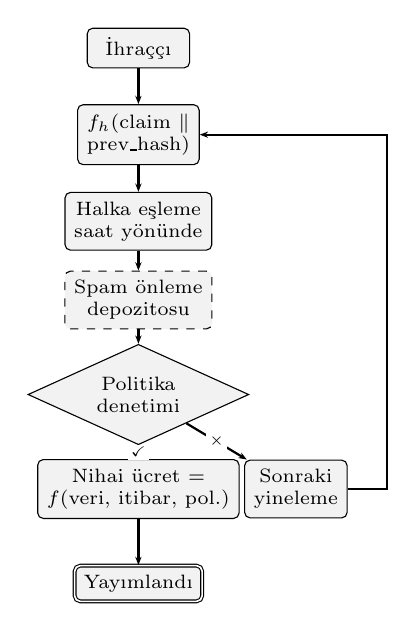
\begin{tikzpicture}[
    box/.style={draw, rounded corners=2pt, minimum width=1.3cm, minimum height=0.45cm, align=center, font=\scriptsize, fill=black!5},
    dec/.style={draw, diamond, aspect=2.2, minimum width=0.9cm, align=center, font=\scriptsize, fill=black!5},
    arr/.style={-{Stealth[length=3pt]}, thick},
    lbl/.style={font=\tiny, fill=white, inner sep=1pt}
]
\node[box] (iss) at (0,0) {İhraççı};
\node[box] (hash) at (0,-1.1) {$f_h$(claim $\|$\\prev\_hash)};
\node[box] (ring) at (0,-2.2) {Halka eşleme\\saat yönünde};
\node[box, dashed] (spam) at (0,-3.2) {Spam önleme\\depozitosu};
\node[dec] (check) at (0,-4.4) {Politika\\denetimi};
\node[box] (rej) at (2,-5.6) {Sonraki\\yineleme};
\node[box] (fee) at (0,-5.6) {Nihai ücret =\\$f$(veri, itibar, pol.)};
\node[box, double] (pub) at (0,-6.8) {Yayımlandı};

\draw[arr] (iss) -- (hash);
\draw[arr] (hash) -- (ring);
\draw[arr] (ring) -- (spam);
\draw[arr] (spam) -- (check);
\draw[arr] (check) -- node[lbl] {$\times$} (rej);
\draw[arr] (check) -- node[lbl] {\checkmark} (fee);
\draw[arr] (fee) -- (pub);
\draw[arr] (rej.east) -- ++(0.5,0) |- (hash.east);
\end{tikzpicture}
\caption{Doğrulayıcı seçim protokolü. Spam önleme depozitosu isteğe bağlıdır ve iade edilebilir. Nihai ücret yalnızca kabul üzerine ödenir.}
\label{fig:verifier}
\end{figure}

Her ret, doğrulayıcının tam yanıtını (gerekçeler ve koşullar dahil) iddia belgesine ekleyerek içeriğini genişletir. Genişletilmiş belgeden, farklı bir halka konumuna eşlenen ve farklı bir doğrulayıcı seçen yeni bir özet deterministik olmayan biçimde hesaplanır. Tam yolun belgelenmesi zorunludur---ihraççı bir sonraki doğrulayıcıyı öngöremez veya etkileyemez. Uyumlu bir beyan edilmiş politikaya rağmen bir doğrulayıcı bir talebi görmezden gelirse, tanıklar (varsa) bunu kaydeder ve ihraççı nihai yayımlama sırasında tanık kanıtı ekleyebilir.

\begin{figure}[ht]
\centering
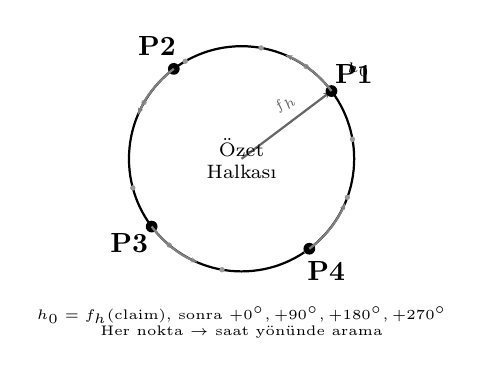
\begin{tikzpicture}[scale=0.65]
% Ring
\draw[thick] (0,0) circle (2.2cm);
% DID nodes on ring
\foreach \a in {10,55,80,120,150,195,230,260,305,340} {
  \fill[black!40] (\a:2.2) circle (1.5pt);
}
% Hash offset arrow pointing to initial position
\draw[-{Stealth[length=3pt]}, thick, black!60] (0,0) -- node[font=\tiny,above,sloped,pos=0.6] {$f_h$} (37:2.2);
\fill[black] (37:2.2) circle (2pt);
\node[font=\tiny,anchor=south west] at (37:2.35) {$h_0$};
% N=4 points offset from h0 by +0, +90, +180, +270
\foreach \offset/\l in {0/P1,90/P2,180/P3,270/P4} {
  \pgfmathsetmacro{\ang}{37+\offset}
  \node[fill=black, circle, inner sep=1.5pt] (p\offset) at (\ang:2.2) {};
  \node[font=\tiny,font=\bfseries] at (\ang:2.75) {\l};
  % clockwise search arc
  \draw[-{Stealth[length=2.5pt]}, thick, gray] (\ang:2.2) arc (\ang:\ang+30:2.2);
}
\node[font=\scriptsize, align=center] at (0,0) {Özet\\Halkası};
\node[font=\tiny, align=center] at (0,-3.2) {$h_0 = f_h(\text{claim})$, sonra $+0^{\circ},+90^{\circ},+180^{\circ},+270^{\circ}$\\Her nokta $\rightarrow$ saat yönünde arama};
\end{tikzpicture}
\caption{Çok noktalı seçim ($N{=}4$). $h_0$ özeti kaymayı belirler; $h_0$'dan eşit dağıtılmış 4 nokta.}
\label{fig:multipoint}
\end{figure}

\subsection{Tanık Protokolü}

\textbf{Tanık} rolü, kriptografik bir meydan okuma kodu protokolü aracılığıyla doğrulayıcı dürüstlüğü için gizli hesap verebilirlik sağlar:

\textbf{Adım W1.} Talep eden, doğrulama talebini imzalar ve $N_w$ tanığa gönderir---talep edenin sosyal ağından kişiler veya ücret karşılığında çalışan uzman tanık hizmeti sağlayıcıları.

\textbf{Adım W2.} Her tanık $w_i$, imzalanmış talebin tamamını imzalar, orijinal imzayı $\sigma_i$ saklar ve bir meydan okuma kodu $c_i = h(\sigma_i)$ hesaplar. Meydan okuma kodu talebe eklenir.

\textbf{Adım W3.} Artık $N_w$ meydan okuma kodu taşıyan talep, doğrulayıcıya gönderilir. Doğrulayıcı kodları görür ancak tanıkların kim olduğunu veya kodların gerçek imzalara karşılık gelip gelmediğini \emph{belirleyemez}.

\textbf{Adım W4 (dürüst doğrulayıcı).} Doğrulayıcı beyan ettiği politikaya göre yanıt verirse, meydan okuma kodları opak kalır. Tanıklar asla açığa çıkmaz. Ek veri yayımlanmaz.

\textbf{Adım W5 (politika ihlali).} Doğrulayıcı politikasını ihlal ederse (talebi görmezden gelir, tutarsız yanıt verir), talep eden tanıkların orijinal imzaları $\sigma_i$'yi elinde tutar. Bunlar yardımcı veri olarak yayımlanabilir: herkes $c_i = h(\sigma_i)$'yi doğrulayabilir ve tanığın hazır bulunduğunu kanıtlayabilir. Talep eden bağımsız olarak yayımlayabilir---doğrulayıcı zaten yanıtında meydan okuma kodlarını imzalamıştır.

\textbf{Blöf özelliği.} Talep eden, meydan okuma kodlarının bazıları veya tümü için rastgele değerler koyabilir. Doğrulayıcı gerçek kodları (yüksek itibarlı otoritelerce desteklenen) gürültüden ayırt edemez. Bu \emph{belirsizlik}, uygulama mekanizmasıdır: her talep, saygın bir otoritenin gizlice izliyor olması riskini taşır. Bu baskıyı sürdürmenin maliyeti sıfıra yakındır (rastgele sayılar üretmek), oysa doğrulayıcı için sahtekârlığın potansiyel maliyeti felakettir. Gerçek tanıkların yokluğunda bile dürüst davranış teşvik edilir.

\textbf{Tanık olarak otorite.} Bir iddiayı onaylayan bir Otorite tanık hizmetlerini birleştirebilir: ``İddianızı onaylıyorum ve doğrulama sırasında gizli tanık olarak hizmet ediyorum.'' Bu doğal bir iş modelidir---Otorite zaten bağlama sahiptir. Ancak iki rol mantıksal olarak bağımsızdır.

\subsection{Pahalı Radikallik İlkesi}

Üç maliyet kanalı aynı anda birleşerek büyür (Şek.~\ref{fig:radicalism}):

\textbf{Kanal 1: Yineleme Maliyeti.} Her ret, zaman ve kaynak tüketen yeni bir yinelemeyi zorunlu kılar. Doğrusal büyüme.

\textbf{Kanal 2: Belge Şişmesi.} Her yineleme, tam doğrulayıcı yanıtını iddia belgesine ekler. Büyüme doğrusaldır ancak bir taban ofsetiyle: başlangıç yükü (iddia içeriği, otorite onayı, kriptografik imzalar) zaten önemsiz olmayan bir $B_0$ boyutuna sahiptir. $k$ yinelemeden sonraki toplam boyut: $S(k) = B_0 + k \cdot \Delta$, burada $\Delta$ ortalama yanıt boyutudur.

\textbf{Kanal 3: Doğrulayıcı Risk Primi.} Risk özneldir. Doğrulayıcı, talep eden DID'in beyan ettiği politikaların doğrulayıcının kendi ticari, sosyal veya siyasî çıkarlarıyla çatışıp çatışmadığını değerlendirir. Prim, doğrulayıcının ``ideali''nden algılanan uzaklıkla üstel olarak yükselebilir: $P(d) = \alpha \cdot e^{\beta d}$, burada $d$ doğrulayıcının öznel uzaklık ölçütüdür. Kişisel bir yasak sınırının ötesinde, doğrulayıcı tamamen reddedebilir.

\begin{figure}[ht]
\centering
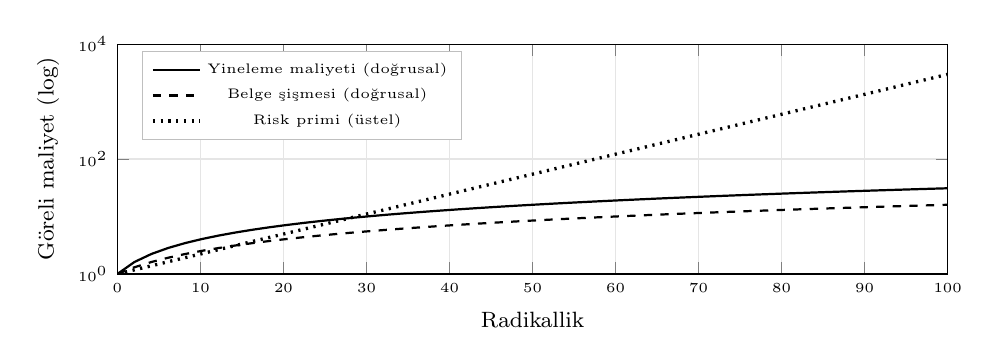
\begin{tikzpicture}
\begin{axis}[
    width=\columnwidth,
    height=4.5cm,
    xlabel={\footnotesize Radikallik},
    ylabel={\footnotesize Göreli maliyet (log)},
    ymode=log,
    xmin=0, xmax=100,
    ymin=1, ymax=10000,
    grid=major,
    grid style={gray!20},
    legend style={at={(0.03,0.97)},anchor=north west,font=\tiny,draw=gray!50},
    tick label style={font=\tiny},
    label style={font=\footnotesize},
]
\addplot[black, thick, domain=0:100, samples=50] {1 + 0.3*x};
\addlegendentry{Yineleme maliyeti (doğrusal)}
\addplot[black, thick, dashed, domain=0:100, samples=50] {1 + 0.15*x};
\addlegendentry{Belge şişmesi (doğrusal)}
\addplot[black, thick, dotted, line width=1.2pt, domain=0:100, samples=100] {exp(0.08*x)};
\addlegendentry{Risk primi (üstel)}
\end{axis}
\end{tikzpicture}
\caption{Üç kanal boyunca maliyet artışı. Risk primi yüksek radikallikte baskın gelir.}
\label{fig:radicalism}
\end{figure}

Kritik olarak, bu sansür değildir. Hiçbir iddia yasaklanmaz. Sistem riski fiyatlandırır (Tablo~\ref{tab:costs}).

\begin{table}[ht]
\centering
\caption{İddia türleri arasında maliyet karşılaştırması.}
\label{tab:costs}
\footnotesize
\begin{tabular}{@{}lcccc@{}}
\toprule
\textbf{Tür} & \textbf{Yin.} & \textbf{Belge} & \textbf{Ücret} & \textbf{Toplam} \\
\midrule
İnandırıcı & $k_{\min}$ & $B_0$ & $P_{\min}$ & Düşük \\
Tartışmalı & $k_{\text{med}}$ & $B_0{+}k\Delta$ & $\alpha e^{\beta d}$ & Orta \\
Radikal & $k_{\max}$ & $\gg B_0$ & $\gg P_{\min}$ & Çok yüksek \\
Sahtekârca & $\to\infty$ & --- & --- & Yayımlanamaz \\
\bottomrule
\end{tabular}
\end{table}

% ============================================================
% 6. REPUTATION AND RISK
% ============================================================
\section{İtibar ve Risk Değerlendirmesi}

\subsection{İtibar Birikim Modeli}

İtibar üç özellik sergiler: \textbf{yavaş birikim} (tutarlı davranışla kademeli büyüme), \textbf{hızlı yıkım} (tek bir sahtekârlık puanı felaket derecesinde düşürebilir) ve \textbf{bireysel değerlendirme} (her tüketici taraf kendi toplama işlevini uygulayabilir).

\subsection{İtibarlı Otoriteler}

Bir İtibarlı Otorite iddiaları inceler ve tatmin olursa onları ortak imzalar---kendi itibarını ortaya koyar (Şek.~\ref{fig:authority}). Asimetri tasarım gereğidir: itibar kazanmak yavaştır (dürüst onay başına kademeli $+\delta$), kaybetmek ise felakettir (sahte onay başına $-\Delta \gg \delta$; örnekleme amacıyla, ör. $+2\%$'ye karşı $-70\%$). Optimal strateji her zaman şüpheli iddiaları reddetmektir. $\delta$ ve $\Delta$'nın özgül değerleri sistem parametreleridir.

\begin{figure}[ht]
\centering
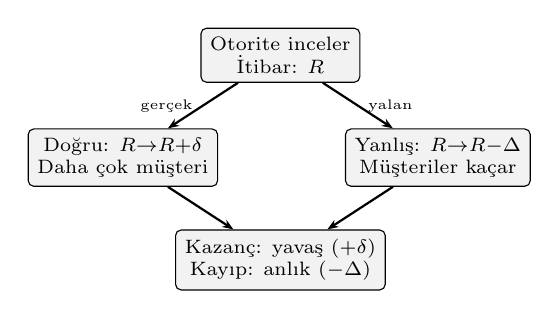
\begin{tikzpicture}[
    box/.style={draw, rounded corners=2pt, minimum width=2cm, minimum height=0.6cm, align=center, font=\scriptsize, fill=black!5},
    arr/.style={-{Stealth[length=4pt]}, thick}
]
\node[box] (exam) at (0,0) {Otorite inceler\\İtibar: $R$};
\node[box] (true) at (-2,-1.3) {Doğru: $R{\to}R{+}\delta$\\Daha çok müşteri};
\node[box] (false) at (2,-1.3) {Yanlış: $R{\to}R{-}\Delta$\\Müşteriler kaçar};
\node[box] (insight) at (0,-2.6) {Kazanç: yavaş ($+\delta$)\\Kayıp: anlık ($-\Delta$)};

\draw[arr] (exam) -- node[left,font=\tiny] {gerçek} (true);
\draw[arr] (exam) -- node[right,font=\tiny] {yalan} (false);
\draw[arr] (true) -- (insight);
\draw[arr] (false) -- (insight);
\end{tikzpicture}
\caption{İtibarlı Otorite---asimetrik teşvikler.}
\label{fig:authority}
\end{figure}

\subsection{Çok Boyutlu İtibar}

İtibar bir skaler değil, birden çok boyutta bir vektördür: malî güvenilirlik, kişisel dürüstlük, mesleki yeterlilik, sivil katılım ve diğerleri (Şek.~\ref{fig:reputation-radar}). Farklı değerlendirme sağlayıcıları bu vektörü bağlama bağlı olarak farklı biçimde yansıtır---bir kredi veren malî güvenilirliği önceler, bir işveren mesleki yeterliliği, bir komşu sivil davranışı. Tek bir ``doğru'' itibar puanı yoktur; yalnızca bakış açıları vardır.

\begin{figure}[ht]
\centering
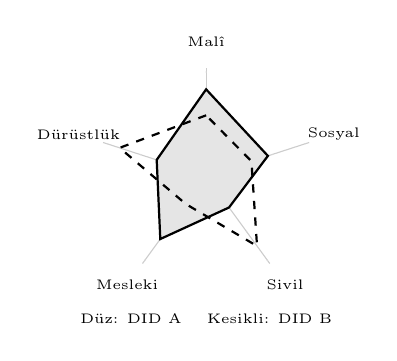
\begin{tikzpicture}[scale=0.55]
\foreach \a/\l in {90/Malî,162/Dürüstlük,234/Mesleki,306/Sivil,18/Sosyal} {
  \draw[gray!40] (0,0) -- (\a:2.5);
  \node[font=\tiny, align=center] at (\a:3.1) {\l};
  \foreach \r in {0.8,1.6,2.4} {
    \fill[black!15] (\a:\r) circle (0.5pt);
  }
}
\draw[thick, fill=black!10] (90:2.0) -- (162:1.2) -- (234:1.8) -- (306:0.9) -- (18:1.5) -- cycle;
\draw[thick, dashed] (90:1.4) -- (162:2.1) -- (234:0.8) -- (306:2.0) -- (18:1.1) -- cycle;
\node[font=\tiny] at (0,-3.3) {Düz: DID A \quad Kesikli: DID B};
\end{tikzpicture}
\caption{Çok boyutlu itibar vektörleri. Farklı DID'ler boyutlar arasında farklı profiller sergiler.}
\label{fig:reputation-radar}
\end{figure}

\subsection{Demokratikleştirilmiş Risk Değerlendirmesi}

RSN, sistematik risk değerlendirmesini demokratikleştirir---şu anda malî kurumlarda yoğunlaşan ancak bankacılığın çok ötesinde uygulanabilir bir yetenek. Tedarikçi güvenilirliğini değerlendiren sınai holdingler, davranışsal riski fiyatlandıran sigorta şirketleri, birleşme ve devralmalar için durum tespiti, imalatta ekipman ömrü tahmini---karşı taraf riskinin değerlendirilmesi gereken her yerde RSN, merkeziyetsiz, piyasa güdümlü bir alternatif sağlar. Bir yorum hizmetleri piyasası, ham çok boyutlu itibar verilerini eyleme geçirilebilir özetlere çevirir ve karşı taraf değerlendirmesini herhangi bir katılımcı için marjinal maliyetle erişilebilir kılar.

% ============================================================
% 7. CONSENSUS AND DISPUTE RESOLUTION
% ============================================================
\section{Uzlaşı ve Uyuşmazlık Çözümü}

\subsection{Merkeziyetsiz Adalet Modeli}

RSN, adaleti iki yönlü bir pazarlık sorunu olarak yeniden çerçeveler. Kalıcı, doğrulanabilir itibar zararı tehdidi, zarar gören tarafın karşılayamayacağı yasal süreçlerden daha etkili bir caydırıcıdır.

\subsection{Kendiliğinden Oluşan Uzlaşı}

Her katılımcı kişisel bir tatmin eşiği tutar. Ağın toplu uzlaşısı, binlerce iki yönlü pazarlığın istatistiksel ortalaması olarak ortaya çıkar (Şek.~\ref{fig:consensus}). Uzlaşının çok üzerinde bir yanıt (barbarca) yayımlaması pahalıdır. Uzlaşıya yakın bir yanıt (orantılı) ucuzdur. Uzlaşı bir kural değildir---bir fiyat sinyalidir.

\begin{figure}[ht]
\centering
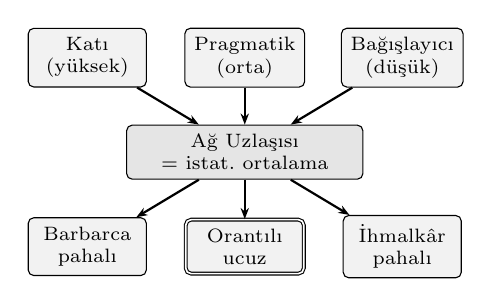
\begin{tikzpicture}[
    person/.style={draw, rounded corners=2pt, minimum width=1.5cm, minimum height=0.5cm, align=center, font=\scriptsize, fill=black!5},
    arr/.style={-{Stealth[length=4pt]}, thick}
]
\node[person] (a) at (-2,0) {Katı\\(yüksek)};
\node[person] (b) at (0,0) {Pragmatik\\(orta)};
\node[person] (c) at (2,0) {Bağışlayıcı\\(düşük)};
\node[person, fill=black!10, minimum width=3cm] (cons) at (0,-1.2) {Ağ Uzlaşısı\\= istat.\ ortalama};
\node[person] (exp) at (-2,-2.4) {Barbarca\\pahalı};
\node[person, double] (prop) at (0,-2.4) {Orantılı\\ucuz};
\node[person] (neg) at (2,-2.4) {İhmalkâr\\pahalı};

\draw[arr] (a) -- (cons);
\draw[arr] (b) -- (cons);
\draw[arr] (c) -- (cons);
\draw[arr] (cons) -- (exp);
\draw[arr] (cons) -- (prop);
\draw[arr] (cons) -- (neg);
\end{tikzpicture}
\caption{Bireysel tatmin eşiklerinden kendiliğinden oluşan uzlaşı.}
\label{fig:consensus}
\end{figure}

\subsection{Cezanın Ayarlanması}

Her DID Sahibi belirli kötü davranış kategorilerine yönelik yanıtlarını kamuya açık olarak beyan eder. Orantısız derecede sert veya hoşgörülü beyanlar olumsuz itibar sinyalleri çeker. Orantılı beyanlar sürtünmesiz kabul edilir---kendini kalibre eden bir ceza sistemi.

Uzlaşı beyanları da ikiyüzlülük tespitine tabidir: bir uzlaşı pozisyonuna beyanen bağlanırken tutarsız davranmak, kasıtlı aldatmayı gösterdiği için temeldeki sapmadan daha ağır bir itibar suçu oluşturur.

\subsection{Devir}

Bir DID içindeki tüm etkinlikler---bir istisna dışında---başka bir DID'e devredilebilir. \textbf{Özne rolü---davranışı iddianın konusu olan DID---devredilemez; iddianın atıfta bulunduğu kimlik sahibine devredilemez biçimde bağlıdır.} Diğer etkin roller---İhraççı, Otorite, Tanık, Doğrulayıcı---ister doğrulama, ister iddia sunma, ister uzlaşı katılımı, ister uyuşmazlık çözümü için olsun, belirlenmiş bir vekil DID'e aktarılabilir. Devir her an geri alınabilir. Bu, Sahibin nihai denetimi ve sorumluluğu elinde tutmasını sağlarken uzmanlaşmaya (ör. profesyonel doğrulama hizmetleri) olanak tanır. Devir tüm sistem boyunca geçerlidir ve ölçeklenebilirlik için elzemdir.

\subsection{Bireysel Ahlaktan Kendiliğinden Oluşan Toplumsal Sözleşmeye}

Her DID'in beyan ettiği politika, bireysel ahlakın bir formülleştirmesini temsil eder: Sahibin neyi kabul edilebilir gördüğü, belirli davranışlara nasıl yanıt verdiği, karşı taraflardan ne talep ettiği. Bu politikalar bir sistem tasarımcısı tarafından dayatılmaz---her katılımcı tarafından seçilir ve makinece okunabilir biçimde ifade edilir.

Bu formülleştirme üç aşamalı bir kendiliğinden oluşumu mümkün kılar. Birincisi, bireysel ahlak \textbf{politika} olarak kodlanır---DID'in uymayı taahhüt ettiği beyan edilmiş kurallar, eşikler ve yanıt işlevleri dizisi. İkincisi, ağdaki tüm politikaların toplamı \textbf{kendiliğinden oluşan etiği} üretir---tek bir katılımcının tasarlamadığı ancak binlerce bireysel ahlakî pozisyonun etkileşiminden doğan, istatistiksel olarak gözlemlenebilir normlar~\cite{durkheim1893}. Üçüncüsü, iki yönlü fiyat sinyalleri aracılığıyla uygulanan paylaşılan davranış normları olarak ifade edilen bu kendiliğinden oluşan etik, \textbf{ölçülebilir bir toplumsal sözleşme} oluşturur---kimsenin imzalamadığı teorik bir kurgu değil~\cite{rawls1971}, gerçek davranışla desteklenen, ampirik olarak gözlemlenebilir bir kurallar dizisi.

Bu süreç ahlakî temeller kuramının bulgularını yansıtır~\cite{haidt2012}: insan ahlakı sezgisel, çoğulcu ve kültürel olarak değişkendir. RSN bir girdi olarak ahlakî uzlaşı gerektirmez; bir çıktı olarak davranışsal uzlaşı üretir. Ortaya çıkan toplumsal sözleşme statik değildir---katılımcılar katıldıkça, ayrıldıkça ve ağ geri bildirimine yanıt olarak politikalarını ayarladıkça evrilir. Klasik toplumsal sözleşme kuramının aksine, bu sözleşme geri alınabilir, gözlemlenebilir ve bir hükümdar olmaksızın uygulanabilirdir.

% ============================================================
% 8. ECONOMIC MODEL
% ============================================================
\section{Ekonomik Model}

Önceki bölümler bir aracı---RSN'nin doğrulama mekanizmalarını, maliyet yapısını ve kendiliğinden oluşan uzlaşısını---tanımladı. Bu bölüm, bu aracın malî ve yönetimsel geçişe uygulanması için bir metodoloji tanımlar. Araç genel amaçlıdır; aşağıdaki metodoloji olası bir uygulamadır.

\subsection{Teşvik Yapısı}

Sermaye olarak itibar, dürüst davranış için doğrudan teşvikler oluşturur. Normal işleyişte katılımcılar itibarı günlük işlemler ve yerine getirilen taahhütler yoluyla doğal olarak oluşturur. Birincil harcama \emph{olumsuz} iddialaradır---başkalarının verdiği zararı kaydetmek. Bu asimetri, yararlı, güvenilir davranışı teşvik eder: dürüst olmanın ek maliyeti yoktur, zararlı olmak ise başkalarının korumak için ödeme yapacağı belgelenmiş bir iz oluşturur. İkiyüzlülük---kurallara uymadan onları beyan etmek---kasıtlı aldatmayı gösterdiği için en maliyetli başarısızlık biçimidir.

\subsection{Paralel Malî Sistem}

Üç bileşen rekabetçi baskı sağlar: (1)~\textbf{Basit Vergi}---istisnasız, tek oranlı, başlangıçta mevcut fiilî oranın marjinal olarak altında bir orantılı vergi; (2)~\textbf{Elektronik Harcama Kaydı (ESR)}---Çek EET modelini tersine çevirerek vatandaşların devlet harcamalarını denetlemesini sağlar; (3)~\textbf{Vatandaş Yönlendirmeli Vergi Tahsisi}---ilk yılda birkaç yüzde ile başlar ve on yıl sonra, benimseme hızına bağlı olarak düşük çift haneli rakamlardan vatandaş yönlendirmeli bir sisteme tam geçişe kadar herhangi bir yere ulaşır. Fiilî tempo, devlet hizmetlerine serbest piyasa alternatiflerinin ortaya çıkma hızına ve devletin geçişle iş birliği yapma isteğine bağlıdır; zamanın işlevinin doğrusal olması gerekmez ve benimsemenin nihayetinde nereye varabileceğine bir üst sınır koymak için hiçbir neden yoktur.

% ============================================================
% 9. MIGRATION PATH
% ============================================================
\section{Geçiş Yolu}

Geçiş üç aşamadan geçer (Şek.~\ref{fig:migration}): \textbf{Aşama~1: Örtü} (bilgi katmanı olarak RSN, devlet tek sağlayıcı), \textbf{Aşama~2: Rekabet} (RSN işlevsel alternatifler sağlar, çift sistem kullanımı) ve \textbf{Aşama~3: Geçiş} (RSN devlet eşdeğerlerinden daha iyi performans gösterir, gönüllü göç). Geçiş her aşamada geri döndürülebilirdir.

\begin{figure}[ht]
\centering
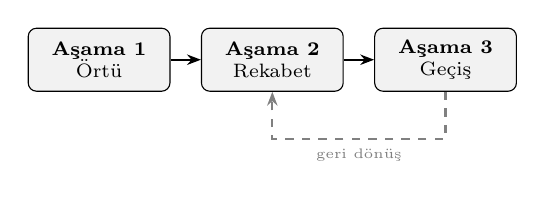
\begin{tikzpicture}[
    phase/.style={draw, rounded corners=3pt, minimum width=1.8cm, minimum height=0.8cm, align=center, font=\scriptsize, fill=black!5},
    arr/.style={-{Stealth[length=5pt]}, thick}
]
\node[phase] (p1) at (0,0) {\textbf{Aşama 1}\\Örtü};
\node[phase] (p2) at (2.2,0) {\textbf{Aşama 2}\\Rekabet};
\node[phase] (p3) at (4.4,0) {\textbf{Aşama 3}\\Geçiş};

\draw[arr] (p1) -- (p2);
\draw[arr] (p2) -- (p3);
\draw[arr, dashed, gray] (p3.south) -- ++(0,-0.6) -| node[below,font=\tiny,pos=0.25] {geri dönüş} (p2.south);
\end{tikzpicture}
\caption{Üç aşamalı geçiş---her aşamada geri döndürülebilir.}
\label{fig:migration}
\end{figure}

Birincil baskı mekanizması malîdir: koşullu vergi mükellefleri ``ekonomik olarak önemli bir azınlık $X$''e ulaştığında---ona karşı baskı önemsiz olmayan ekonomik zarara yol açacak ve sivil itaatsizliğin inandırıcı bir tehdit haline geleceği kadar büyük bir grup---devlet müzakereye girer. Örnekleme amacıyla $X \approx 15\%$ (GSYİH'nin) kullanıyoruz, ancak fiilî eşik belirli ekonomiye bağlıdır.

% ============================================================
% 10. SECURITY ANALYSIS
% ============================================================
\section{Güvenlik Analizi}

Beş düşman kategorisini ele alıyoruz: bireysel kötü niyetli aktörler, örgütlü gruplar, kurumsal düşmanlar, devlet düzeyindeki düşmanlar ve protokol düzeyindeki düşmanlar.

\textbf{Sybil direnci}~\cite{douceur2002}. İtibar oluşturmak, sürekli, doğrulanabilir etkileşim gerektirir. Başarılı bir Sybil saldırısının maliyeti, sahte kimliklerle doğrusal ve hedef itibar düzeyiyle karesel olarak ölçeklenir. Paralel olarak birden çok DID işletmek mümkündür ancak tasarım gereği pahalıdır---her kimlik, gerçek etkinlik yoluyla bağımsız olarak itibar biriktirmelidir. Özgür toplumlarda bu maliyet gelişigüzel istismarı caydırır; diktatörlüklerde ise paralel DID'ler, bölmelenmiş direnişi, yeraltı koordinasyonunu ve daha güvenli karaborsa gezinmesini mümkün kılan bir hayatta kalma aracı haline gelir.

\textbf{Gizli anlaşma savunması.} Kapalı gruplar arasındaki karşılıklı onay örüntüleri, sosyal grafik analizi yoluyla tespit edilebilir. İtibar toplama işlevleri, sıkı biçimde kümelenmiş kaynaklardan gelen iddiaları iskonto eder.

\textbf{Devlet düzeyinde düşman.} Soğan yönlendirmesi, merkezî altyapının yokluğu ve Doğrulayıcı rolünün katılımcı tabanına dağıtılması, bastırmanın herhangi bir yararla orantısız önlemler gerektirmesini sağlar.

\textbf{Mahremiyete karşı hesap verebilirlik.} Takma adlılık---anonimlik ile kimlik ifşası arasında bir orta yol---DID'lerin Sahibin gerçek dünyadaki kimliğini açığa çıkarmadan anlamlı itibar biriktirmesine olanak tanır.

% ============================================================
% 11. PRIVACY
% ============================================================
\section{Mahremiyet Değerlendirmeleri}

RSN'nin mahremiyet modeli takma adlılık üzerine kuruludur. Sahip kimlik ifşasını denetler: asgari (saf takma ad), seçici (belirli kimlik bilgileri bağlı) veya tam (yasal kimlik ilişkilendirilmiş). Yayımlanan iddialar kalıcıdır---sistem bağlamsal düzeltmeyi destekler ancak silmeyi desteklemez. Bir Sahip, biriktirilen itibarı feda ederek tehlikeye girmiş bir DID'i terk edip yeniden başlayabilir.

% ============================================================
% 12. RELATED WORK
% ============================================================
\section{İlgili Çalışmalar}

W3C DID Core spesifikasyonu~\cite{did2022} ve Ceramic Network~\cite{ceramic2023} kimlik temelini sağlar. EigenTrust~\cite{kamvar2003} merkezî otorite olmaksızın dağıtık itibar toplamasını gösterdi. SBT'ler~\cite{weyl2022} devredilemez sosyal belirteçleri tanıttı. RSN, bir kalite filtresi olarak ekonomik maliyete vurgusu ve radikalliği fiyatlandırma mekanizmasıyla farklılaşır.

DAO'lar~\cite{buterin2014} ve karesel oylama~\cite{buterin2019} merkeziyetsiz yönetimin uygulanabilirliğini gösterdi. RSN uzlaşıyı oylamadan ziyade iki yönlü fiyat pazarlıklarından türetir.

Öneri, özel hizmet sağlama için anarko-kapitalist kuramdan~\cite{rothbard1973,hoppe2001} yararlanır ancak iki kritik açıdan ayrılır: rasyonellik varsaymak yerine kin ve intikam dürtüleri için tasarım yapar ve devrim yerine kademeli geçiş önerir. Kendiliğinden oluşan toplumsal sözleşmeler kavramının, Hayek'in kendiliğinden düzen kuramında~\cite{hayek1973} öncülleri vardır.

\textbf{Anarko-agorizm.} RSN, agorist karşı-ekonomi ile~\cite{konkin2006}---özellikle paralel kurumlar inşa etmeye ve gönüllü değişime yaptığı vurguyla---önemli bir ortak zemin paylaşır. Ancak agorizm, rasyonel öz-çıkarı yeterli bir koordinasyon mekanizması olarak varsayma eğilimindedir ve genellikle mevcut devlet yapılarından somut bir geçiş yolundan yoksundur. RSN, rasyonel olmayan davranışsal eğilimleri açıkça bünyesine katar ve kademeli geçiş için malî bir baskı mekanizması sağlar.

\textbf{Liyakat sistemi.} RSN, liyakatin~\cite{young1958} bir slogan yerine sistemik bir özellik olarak nasıl ortaya çıkabileceğine dair ilk işlevsel tanımı temsil edebilir. Geleneksel liyakat sistemleri başarısız olur çünkü ``liyakati'' tanımlayacak ve uygulayacak merkezî bir otorite gerektirir. RSN'de liyakat iki yönlü değerlendirmelerden ortaya çıkar: değer sunanlar itibar biriktirir; kimin liyakatli olduğuna hiçbir komite karar vermez.

\textbf{Ayrıcalık olarak mülkiyet.} RSN, mülkiyet haklarına doğal ve mutlak olarak yaklaşan anarko-kapitalist ve Avusturya okulu yaklaşımlarından temelde ayrılır. RSN çerçevesinde mülkiyet bir \emph{ayrıcalıktır}---bir katılımcı paylaşılan normları temelden ihlal ettiğinde (ihanet, varoluşsal krizde topluluğu savunmayı reddetme, sistematik sömürü) uç durumlarda topluluk tarafından geri çekilebilen bir toplumsal tanınma. Bu, devlet kamulaştırması değil, iki yönlü ilişkiler ağı tarafından toplumsal tanınmanın geri çekilmesidir.

% ============================================================
% 13. LIMITATIONS
% ============================================================
\section{Tartışma ve Sınırlamalar}

\textbf{Soğuk başlangıç.} RSN'nin değeri ağ etkilerine bağlıdır; erken benimseyenler, katılım bir eşiğe ulaşana dek sınırlı değerle karşı karşıya kalır. Ancak erken aşamalardan itibaren bile DID ağı yararlı bir tamamlayıcı bilgi kaynağı olarak hizmet eder. Erken itibar değerlendirmesi ve otorite değerlendirmesinin artan gelişmişlikle kademeli olarak gelişmesi beklenir.

\textbf{Asalaklığı önleme ve erişim denetimi.} Hedef DID'ler, düşük itibarlı DID'lerden gelen sorgulara kademeli ücretler ve erişim kısıtlamaları getirebilir. Bu ikili değil sürekli bir ölçektir: sorgulayan bir DID'in itibarı ne kadar azsa, o kadar az bilgi alır, o kadar uzun bekler ve o kadar çok öder. Bu mekanizma, edilgen tüketim yerine gerçek katılımı teşvik eder.

\textbf{Erişim eşitsizliği.} İddia yayımlama maliyeti, ekonomik olarak dezavantajlı katılımcıların meşru şikâyetlerini süzebilir. Hafifletme: her katılımcı aynı zamanda potansiyel bir doğrulayıcı olarak hizmet eder (veya bu rolü devreder) ve doğrulama ücretleri kazanır. Yeterli bir zaman ufkunda, radikal olmayan bir katılımcı malî tarafsızlığa yaklaşmalıdır---doğrulama geliri yayımlama maliyetlerini yaklaşık olarak dengeler. Bu bir garanti değil, istatistiksel bir beklentidir.

\textbf{İtibar eşitsizliği.} Erken benimseyenler, geç kalanlar için engeller oluşturabilecek avantajlar biriktirir. Ancak itibar değerlendirmesi, toplama algoritmaları aracılığıyla ilk hamle avantajını hafifletmeyi seçebilecek üçüncü taraf sağlayıcılar tarafından yapılır. İyi bir itibarla ilk olmak meşru bir karşılaştırmalı ekonomik avantajdır---ve bu tasarım gereğidir.

\textbf{Açık sorular.} Optimal maliyet işlevleri, toplama standartları, protokol yönetimi ve yapay zekâ tarafından üretilen sentetik itibar verileriyle etkileşim gelecekteki çalışma alanları olarak kalır.

Bu makale, RSN'nin her koşulda optimal sonuçlar üreteceğini iddia etmez. RSN'nin \emph{uygulanabilir} bir alternatif temsil ettiğini iddia eder---teknik olarak uygulanabilir, ekonomik olarak kendi kendini sürdürebilir ve insan davranış eğilimleriyle gerçekte oldukları haliyle sosyal olarak uyumlu.

% ============================================================
% 14. CONCLUSION
% ============================================================
\section{Sonuç}

Bu makale, takma adlı, doğrulanabilir itibar değişimini mümkün kılan merkeziyetsiz bir protokol olan İtibar Sosyal Ağı'nı sundu. Pahalı Radikallik İlkesi, sahtekârca iddiaların sansür olmaksızın fiyat yoluyla dışlanmasını sağlar. Önerilen geçiş yolu, mevcut kurumlardan kademeli, geri döndürülebilir bir geçişi mümkün kılar. Tasarım, ideolojik dönüşüm gerektirmek yerine insan doğasını olduğu haliyle---küçüklük, kin ve intikam alma tatmini arzusu dahil---bünyesine katar. Sonuç bir ütopya değil, adaletin erişilebilir olduğu, itibarın hak edildiği ve kötü davranışın maliyetinin ona neden olan tarafça üstlenildiği bir sistemdir.

% ============================================================
% REFERENCES
% ============================================================
\bibliography{references}

\end{document}
